\documentclass[./main.tex]{subfiles}


\begin{document}

\newcommand{\ob}{\textit{1B} }
\newcommand{\fb}{$\forall$\textit{1B} }
\newcommand{\cb}{\textit{CB} }
\newcommand{\dbb}{\textit{DB} }

\chapter{Implementazione di procedure di decisione per frammenti Binding in Vampire}

(descrizione dell'approccio, minime modifiche al kernel, utilizzo di funzionalità esistenti,)

\section{Algoritmo di Classificazione}

\begin{figure}[H]
    \centering
    \scalebox{0.55}{
        \includesvg{images/4_progettazione/Classifier.svg}
    }
    \caption{Classificatore}
    \label{fig:classifier}
\end{figure}

La precondizione più importante per la correttezza dell'algoritmo di decisione è che la formula faccia parte del frammento $\forall1B$.
Per questo motivo è stato creato un classificatore che prende in input una formula rettificata e restituisce l'elemento del frammento a cui appartiene.
Una formula è rettificata se non contiene $\top$ o $\bot$. 
L'algoritmo non fa altro che verificare la forma sintattica della formula e capisce a quale grammatica della sezione \ref{sec:binding_taxonomy}
appartiene. Per questo scopo sono state create due funzioni delle Classificatore Esterno (Algoritmo \ref{alg:classifier}) e Classificatore Interno (Algoritmo \ref{alg:innerClassifier}).
La prima verifica la parte della formula senza quantificatori mentre la seconda verifica la parte interna ai quantificatori e confronta 
i termini dei letterali. 
Entrambi gli algoritmi hanno una struttura di visita dell'albero sintattico in postOrder e hanno una complessità lineare rispetto alla dimensione della formula.


\begin{algorithm}[H] \label{alg:classifier}
\caption{Classificatore esterno}
\KwSty{Firma:}{ classify($\varphi$)}
\KwIn{$\varphi$ Una formula rettificata}
\KwOut{Un elemento dell'enumerazione Fragment}

\Switch{$\varphi$}{
    \Case{$Literal$}{
        \Return ONE\_BINDING\;
    }
    \Case{$A [\land, \lor] B$}{
        \Return $compare(classify(A), classify(B))$\;
    }
    \Case{$\lnot A$}{
        \Return $classify(A).complementary()$\;
    }
    \Case{$[\forall, \exists]A$}{
        $sub := \varphi$\;
        $connective := \text{connective of } \varphi$\;
        \Repeat{$connective \notin \{\forall, \exists\}$}{
            $sub := \text{subformula of sub}$\;
            $connective := \text{connective of sub}$\;
        }
        $(fragment, \_) := innerClassify(sub)$\;
        \Return $fragment$\;
    }

    \Case{$A \Leftrightarrow B$}{
        \Return $compare(classify(A \Rightarrow B), classify(B \Rightarrow A))$\;
    }
    \Case{$A \oplus B$}{
        \Return $classify(A \Leftrightarrow B).complementary()$\;
    }
    \Case{$A \Rightarrow B$}{
        \Return $compare(classify(\lnot A), classify(B))$\;
    }
}
\end{algorithm}
\begin{algorithm}[H] \label{alg:compare}
    \caption{Compare esterno}
    \KwSty{Firma:}{ compare($A, B$)}
    \KwIn{$A, B$ due elementi dell'enumerazione Fragment}
    \KwOut{Un elemento dell'enumerazione Fragment}
\If{$A = B$}{
    \Return $A$\;
}
\If{$One\_Binding \notin \{A, B\}$}{
    \Return $None$\;
}
\Return $max(A, B)$\;

\end{algorithm}

Il classificatore esterno si appoggia ad una funzione ausiliaria chiamata \textit{compare} che prende in input due elementi 
dell'enumerazione Fragment e restituisce il frammento risultante dalla combinazione booleana ($\land, \lor$) dei due frammenti.
La combinazione di due \ob è sempre un \ob mentre la combinazione di un \ob con un \cb o \dbb è sempre un \cb o \dbb.
Infine la combinazione di un \cb con un \dbb fa parte del frammento Boolean Binding che però in questa sezione verrà chiamato \textit{None}.
Per la comparazione è stato creato un ordinamento dei frammenti che segue una struttura a rombo:

\begin{center}
    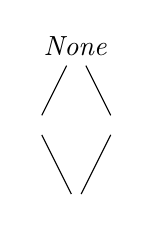
\begin{tikzpicture}
        \node (one) at (0, 0) {\ob};
        \node (conj) at (-0.5, 1) {\cb};
        \node (disj) at (0.5, 1) {\dbb};
        \node (none) at (0, 2) {\textit{None}};
        \draw (one) -- (conj) -- (none) -- (disj) -- (one);
    \end{tikzpicture}
\end{center}

Dove \ob è il minimo e \textit{None} è il massimo.
Il risultato è un reticolo e la funzione compare restituisce l'estremo superiore dei due frammenti.
La funzione complementary restituisce il frammento della negazione di una formula di un determinato frammento.
In particolare il complementare di un \ob è \ob mentre il complementare di un \cb è \dbb e viceversa.



\begin{algorithm}[H] \label{alg:innerClassifier}
    \caption{Classificatore interno}
    \KwSty{Firma:}{ innerClassify($\varphi$)}
    \KwIn{$\varphi$ Una formula rettificata}
    \KwOut{Una coppia (Fragment, Literal)}


\Switch{$\varphi$}{
    \Case{$Literal \; l$}{
        \Return $(ONE\_BINDING, l)$\;
    }
    \Case{$A [\land, \lor] B$}{
        \Return $innerCompare(innerClassify(A), innerClassify(B), \text{connective of } \varphi)$\;
    }
    \Case{$\lnot A$}{
        \Return $innerClassify(A).complementary()$\;
    }
    \Case{$A [\Rightarrow, \Leftrightarrow, \oplus] B$}{
        \Return $innerCompare(innerClassify(A), innerClassify(B), \text{connective of } \varphi)$\;
    }
    \Else{
        \Return $(None, null)$\;
    }
    
}
\end{algorithm}

La struttura del classificatore interno è molto simile a quella del classificatore esterno, mentre il comparatore interno
è leggermente più complesso. Il caso base è quando la formula è un singolo letterale che è sempre un \ob.
La visita in postOrder restituisce una coppia (Fragment, Literal) che rappresenta il frammento a cui appartiene la formula e un letterale
di rappresentanza della formula in questo caso il letterale più a sinistra. 
Il letterale serve a mantenere una reference alla lista di termini delle formule del frammento \ob.

\begin{algorithm}[H] \label{alg:innerCompare}
    \caption{Compare interno}
    \KwSty{Firma:}{ innerCompare($A, B, con$)}
    \KwIn{$A, B$ due coppie (Fragment, Literal), $con$ un connettivo}
    \KwOut{Una coppia (Fragment, Literal)}



    \Switch{A.first, B.first, con}{
        \Case{One\_Binding, One\_Binding, \_\_}{
            \If{$A.second$ has same terms of $B.second$}{
                \Return $A$\;
            } \ElseIf{$conn = \land$}{
                \Return $(Conjunctive\_Binding, null)$\;
            } \ElseIf{$conn = \lor$}{
                \Return $(Disjunctive\_Binding, null)$\; 
            }
        }

        \Case{[One\_Binding, Conjunctive\_Binding $\mid$ Conjunctive\_Binding, One\_Binding], $\land$}{
            \Return (Conjunctive\_Binding, null)\;
        }
        \Case{[One\_Binding, Disjunctive\_Binding $\mid$ Disjunctive\_Binding, One\_Binding], $\lor$}{
            \Return (Disjunctive\_Binding, null)\;
        }

        \Case{Conjunctive\_Binding, Conjunctive\_Binding, $\land$}{
            \Return (Conjunctive\_Binding, null)\;
        }
        \Case{Disjunctive\_Binding, Disjunctive\_Binding, $\lor$}{
            \Return (Disjunctive\_Binding, null)\;
        }
    }

    \Return $(None, null)$\;
\end{algorithm}


La combinazione booleana di due frammenti \ob (all'interno di un quantificatore) può portare 
a tre diversi risultati.
Se i termini dei letterali di rappresentanza sono uguali allora la combinazione è ancora un \ob altrimenti 
la combinazione è un \cb se il connettivo è $\land$ e un \dbb se il connettivo è $\lor$. 
Il termine \textit{null} viene usato come sostituto del letterale di rappresentanza in formule del frammento \cb e \dbb in quanto 
sono una combinazione di più \ob e non hanno un letterale di rappresentanza.
Due frammenti \cb rimangono \cb solo se il loro connettivo è $\land$.
La combinazione di un \ob con un \cb è un \cb se il connettivo è $\land$. Stesso discorso per i \dbb e il connettivo $\lor$.
In tutti gli altri casi la combinazione è \textit{None}. 
Nell'algoritmo \ref{alg:innerCompare} sono stati omessi i casi con connettivi $\Rightarrow, \Leftrightarrow, \oplus$ 
in quanto non sono riconducibili a formule composte da $\land$ e $\lor$ come è stato fatto ad esempio nell'algoritmo \ref{alg:classifier}.
Con la funzione complementary applicata ad una coppia: (Fragment, Literal).complementary() si intende la coppia (Fragment.complementary(), Literal).



\section{Preprocessing}

\begin{figure}[H]
    \centering
    \scalebox{0.55}{
        \includesvg{images/4_progettazione/Preprocess.svg}
    }
    \caption{Struttura del Preprocessing}
    \label{fig:preprocessing}
\end{figure}

In questa sezione verrà descritto l'algoritmo di preprocessing utilizzato per trasformare una formula in input
del frammento \ob o \cb in una struttura trattabile dall'algoritmo di decisione.
Per utilizzare il SatSolver di Vampire per la ricerca degli implicanti è necessario clausificare la formula.
Inoltre per evitare un esplosione esponenziale di formule causate dalle forme NNF e CNF è necessario utilizzare tecniche di naming.
Qui sorgono i primi problemi visto che ne la clausificazione ne il naming sono processi conservativi rispetto ai frammenti.
Ad esempio la semplice formula del frammento \ob $\forall x_1 (p_1(x_1)) \lor p_2$ clausificata diventa  $\{\{p_1(x_1), p_2\}\}$ che fa parte del frammento \dbb.
L'approccio utilizzato è stato quello di creare una nuova formula ground che rappresenta la struttura booleana esterna della formula originale,
applicare le funzioni standard di preprocessing
e mantenere una serie di strutture per risalire ai componenti originali.
Per questo scopo viene introdotto un nuovo insieme di simboli di predicato $\Sigma_b = \{b_1, b_2, ...\}$.
I predicati di $\Sigma_b$ con arità 0 saranno chiamati \textit{booleanBinding} e saranno associati ad una formula del frammento \ob o \cb.
I predicati di $\Sigma_b$ con arità $n > 0$ saranno chiamati \textit{literalBindign} e fungeranno da rappresentati dei $\tau$-Binding delle formule \ob.
Il preprocessing seguirà pressochè questa struttura:

\begin{enumerate}
    \item Rettificazione
    \item Trasformazione in ENNF
    \item Creazione della formula booleana esterna (FBE) e associazione dei booleanBinding
    \item Naming della FBE
    \item Trasformazione in NNF della FBE
    \item Creazione dei literalBinding e Sat-Clausificazione delle formule mappate dai booleanBinding
    \item Creazione delle Sat-Clausole della FBE
\end{enumerate}

La rettificazione e la trasformazione in ENNF sono processi conservativi rispetto ai frammenti e quindi verranno applicate 
direttamente le funzioni standard di Vampire.
La creazione della FBE e l'associazione dei booleanBinding avviene tramite l'algoritmo \ref{alg:topBooleanFormula}.

\begin{algorithm}[H] \label{alg:topBooleanFormula}
    \caption{Top Boolean Formula}
    \KwSty{Firma:}{ topBooleanFormula($\varphi$)}\\
    \KwIn{$\varphi$ una formula rettificata}
    \KwOut{Una formula ground}
    \KwSty{GlobalData: }{ bindingFormulas una mappa da booleanBinding a formula}
\Switch{$\varphi$}{

\Case{Literal l}{
    \Return new AtomicFormula(l)\;
}
\Case{A$[\land, \lor]$B}{
    \Return new JunctionFormula(topBooleanFormula(A), connective of $\varphi$, topBooleanFormula(B))\;
}
\Case{$\lnot$A}{
    \Return new NegatedFormula(topBooleanFormula(A))\;
}
\Case{$[\forall, \exists]$A}{
    $b = newBooleanBinding()$\;
    $bindingFormulas[b] := \varphi$\;
    \Return new AtomicFormula(b)\;
}

\Case{A$[\Leftrightarrow, \Rightarrow, \oplus]$B}{
    \Return new BinaryFormula(A, connective of $\varphi$, B)\;
}
}
\end{algorithm}

L'algoritmo prende in input una formula rettificata e restituisce una formula ground sostituendo le sottoformule quantificate con 
un nuovo booleanBinding aggiungendo la sottoformula originale alla mappa bindingFormulas.
Da adesso in poi qualunque modifica fatta alla FBE preserverà l'appartenenza al frammento originale.
Gli step successivi sono quindi applicare le funzioni standard di Vampire per il naming e la trasformazione in NNF.
La trasformazione in NNF potrebbe portare alla negazione di qualche booleanBinding
e va quindi aggiunta alla mappa bindingFormulas la formula negata associata.

\ForEach{$l \in literals(\varphi)$}{
    \If{$\lnot$l.polarity()}{
        \textbf{continue}
    } 
    $positiveFormula := bindingFormulas[positiveLiteral(l)]$\; \\
    $bindingFormulas[l] := new NegatedFormula(positiveFormula)$\;
}

A questo punto inizia il processo di SatClausificazione delle formule interne (quelle associate ai booleanBinding).
Ogni letterale ground che non è un booleanBinding viene trasformato in una 
SatClausola di lunghezza 1 composta dal solo satLetterale associato al letterale.

\ForEach{$l \in literals(\varphi)$}{
    \If{$l$ is not a booleanBinding}{
        $bindingClauses[l] := new SatClause\{toSat(l)\}$\;
    }
}

Per essere clausificate le formule della mappa bindingFormulas vanno trasformate in NNF, Skolemizzate.
Anche in questo caso vengono utilizzate le funzioni standard di Vampire. 
Ogni booleanBinding è associato ad una formula del frammento ConjunctiveBinding,
per questo dopo la skolemizzazione il quantificatore universale viene distribuito sull'and per ottenere le sottoformule del frammento OneBinding.
Per ogni sottoformula OneBinding viene creato un nuovo LiteralBinding in rappresentaza della sottoformula.
Il nuovo letterale avrà gli stessi termini del letterale più a sinistra della sottoformula (che sono gli stessi di tutti i letterali della sottoformula).
Successivamente la formula viene SatClausificata. 
Si aggiunge alla mappa satClauses la coppia composta dal nuovo LiteralBinding e le satClausole della sottoformula.
Alla mappa literalToBooleanBindings viene aggiunta la coppia composta dal nuovo LiteralBinding e il booleanBinding associato mentre alla mappa
booleanBindingToLiteral viene aggiunta la coppia composta dal booleanBinding e la lista dei LiteralBinding che rappresentano le sottoformule della formula originale.  


\While{bindingFormulas $\neq \emptyset$}{
    $(booleanBinding, formula) := bindingFormulas.pop()$\;\\
    $formula := nnf(formula)$\;\\
    $formula := skolemize(formula)$\;\\
    $toDo := \emptyset$\;\\

    \If{formula is ConjunctiveBinding}{
        $formula := distributeForAll(formula)$\;\\
        "Add each subformula to the todo list"\;
    } \Else{
        toDo.add(formula)\;
    }

    $literalBindings := \emptyset$\;
    \While{todo $\neq \emptyset$}{
        $subformula := todo.pop()$\;\\
        $literalBinding := newLiteralBinding(subformula.mostLeftLiteral())$\;\\
        $clauses := SatClausifyBindingFormula(subFormula)$\;\\

        $satClauses[literalBinding] := clauses$\;\\
        $literalToBooleanBindings[literalBinding] := booleanBinding$\;\\
        $literalBindings.add(literalBinding)$\;\\
    }
    $booleanBindingToLiteral[booleanBinding] := literalBindings$\;
}

La funzione SatClausifyBindingFormula è una funzione che prende in input una formula
la clausifica e converte tutte le clausole in SatClausole in modo che ogni satLetterale ha lo stesso indice del funtore del predicato associato.
Questo è differente da quello che viene fatto dalla classe Sat2Fo che associa ogni puntatore a letterale ad un nuovo SatLetterale con un nuovo indice arbitrario.
L'ultimo step è la SatClausificazione della FBE che avviene tramite le funzioni standard di Vampire della classe Sat2Fo.
È importante ricordare che i satLetterali delle formule interne sono diversi dai satLetterali della FBE nonostante possano avere
lo stesso indice.

Si prenda ad esempio la formula del frammento \cb:

$$ (\forall x_1, x_2 ((p_1(x_1) \lor p_2(x_1)) \land p_2(f_1(x_2))) 
\land  \forall x_1 (p_3(x_1) \Rightarrow p1(x_1)))  
\lor (\forall x_1(p_2(x_1)) \Rightarrow p_4)
$$

Il primo passo di preprocessing prevede la rettificazione e la trasformazione in ENNF.
La formula è già rettificata mentre la trasformazione in ENNF porta all'eliminazione del $\Rightarrow$:

$$ (\forall x_1, x_2 ((p_1(x_1) \lor p_2(x_1)) \land p_2(f_1(x_2))) 
\land  \forall x_1 (\lnot p_3(x_1) \lor p1(x_1)))  
\lor (\forall x_1(p_2(x_1)) \Leftrightarrow p_4)
$$

La creazione della FBE porta alla generazione di un booleanBinding per ogni sottoformula quantificata:

$$ (b_1 
\land  b_2)  
\lor (b_3 \Leftrightarrow p_4)
$$

La mappa bindingFormulas contiene le seguenti coppie:

\begin{itemize}
    \item [$b_1$] $\rightarrow \forall x_1, x_2 ((p_1(x_1) \lor p_2(x_1)) \land p_2(f_1(x_2))) $
    \item [$b_2$] $\rightarrow \forall x_1 (\lnot p_3(x_1) \lor p1(x_1))$
    \item [$b_3$] $\rightarrow \forall x_1(p_2(x_1))$
\end{itemize}

La formula ottenuta è troppo piccola per poter applicare il namig
quindi si procede direttamente con la trasformazione in NNF:

$$ (b_1 
\land  b_2)  
\lor ((\lnot b_3 \lor p_4) \land (b_3 \lor \lnot p_4))
$$

Durante il processo di NNF il booleanBinding $b_3$ è stato negato e quindi va aggiunto alla mappa bindingFormulas:

\begin{itemize}
    \item [$\lnot b_3$] $\rightarrow \exists x_1(\lnot p_2(x_1))$
\end{itemize}

A questo punto vengono trasformate in NNF e Skolemizzate le formule associate ai booleanBinding,
vengono poi creati i literalBindings e le SatClausole delle formule interne.
Il booleanBinding $b_1$ è associato ad una formula \cb quindi 
viene distribuito il quantificatore universale sull'and e creati due literalBindings.
La skolemizzazione della formula associata a $\lnot b_3$ porta alla formula::
\begin{itemize}
    \item [$\lnot b_3$] $\rightarrow \lnot p_2(sk_1)$
\end{itemize}
Vengono create così le mappe booleanBindingToLiteral e la sua inversa literalToBooleanBindings:

\begin{table}[H]
    \centering
    \begin{tabular}{|c|c|}
        \hline
        \textbf{booleanBindingToLiteral} & \textbf{literalToBooleanBindings} \\
        \hline
        $b_1 \rightarrow \{b_4(x_1), b_5(f_1(x_1))\}$ & $b_4(x_1) \rightarrow b_1$\\
        $b_2 \rightarrow \{b_6(x_1)\}$ & $b_5(f_1(x_1)) \rightarrow b_1$ \\
        $b_3 \rightarrow \{b_7(x_1)\}$ & $b_6(x_1) \rightarrow b_2$ \\
        $\lnot b_3 \rightarrow \{b_8(sk_1)\}$ & $b_7(x_1) \rightarrow b_3$ \\
        & $b_8(sk_1) \rightarrow \lnot b_3$ \\
        \hline
    \end{tabular}
\end{table}

Le formule associate ai literalBindings vengono clausificate:

\begin{itemize}
    \item $\forall x_1, x_2 ((p_1(x_1) \lor p_2(x_1))) \rightarrow \{\{(p_1(x_1), p_2(x_1))\}\}$
    \item $\forall x_1, x_2 (p_2(f_1(x_2))) \rightarrow \{\{p_2(f_1(x_2))\}\}$
    \item $\forall x_1 (\lnot p_3(x_1) \lor p1(x_1)) \rightarrow \{\{\lnot p_3(x_1), p1(x_1)\}\}$
    \item $\forall x_1(p_2(x_1)) \rightarrow \{\{p_2(x_1)\}\}$
    \item $\lnot p_2(sk_1) \rightarrow \{\{\lnot p_2(sk_1)\}\}$
\end{itemize}

E successivamente SatClausificate e associate ai literalBindings:
\begin{itemize}
    \item $b_4(x_1) \rightarrow \{\{s_1, s_2\}\}$
    \item $b_5(f_1(x_1)) \rightarrow \{\{s_2\}\}$
    \item $b_6(x_1) \rightarrow \{\{\lnot s_3, s_1\}\}$
    \item $b_7(x_1) \rightarrow \{\{s_2\}\}$
    \item $b_8(sk_1) \rightarrow \{\{\lnot s_2\}\}$
\end{itemize}

Gli ultimi due step sono la clausificazione della FBE:
$$ \{\{b_1, \lnot b_3, p_4\}, \{b_2, \lnot b_3, p_4\}, \{b_1, b_3, \lnot p_4\}, \{b_2,  b_3, \lnot p_4\}\} $$
E la SatClausificazione tramite sat2Fo:
$$ \{\{s_1, \lnot s_2, s_3\}, \{s_4, \lnot s_2, s_3\}, \{s_1, s_2, \lnot s_3\}, \{s_4,  s_2, \lnot s_3\}\} $$
Che crea internamente una bi-mappa che associa ogni satletterale ad un letterale:
\begin{multicols}{2}
\begin{itemize}
    \item $s_1 \leftrightarrow b_1$
    \item $s_2 \leftrightarrow \lnot b_3$
    \item $s_3 \leftrightarrow p_4$
    \item $s_4 \leftrightarrow b_2$
\end{itemize} 
\end{multicols}



\section{Procedura di Decisione}
\begin{figure}[H]
    \centering
    \scalebox{0.55}{
        \includesvg{images/4_progettazione/OneBindingAlgorithm.svg}
    }
    \caption{Struttura dell'algoritmo di decisione}
    \label{fig:algoritmo_decisione}
\end{figure}

\subsection{Implicants Sorting}
\subsection{Maximal Unifiable Subsets}


\begin{algorithm}[H]
    \caption{Maximal Unifiable Subsets}
    \KwSty{Firma:}{ mus($literal$)}\\
    \KwIn{$literal$ un puntatore ad un letterale}
    \KwOut{$\top$ o $\bot$}
    \KwSty{GlobalData: }{ S una mappa da letterali a bool}

\If{$S[literal]$}{
    \Return $\top$\;
}
\If{$literal$ is ground}{
    \Return $groundLiteralMus(literal)$\;
}

$S[literal] = \top$\;
$res := mus(literal, \emptyset)$\;
$S[literal] = \bot$\;
\Return $res$\;
\end{algorithm}


\begin{algorithm}[H]
    \caption{Maximal Unifiable Subsets}
    \KwSty{Firma:}{ mus($literal$, $FtoFree$)}\\
    \KwIn{$literal$ un puntatore ad un letterale, $FtoFree$ un puntatore ad una lista di letterali}
    \KwOut{$\top$ o $\bot$}
    \KwSty{GlobalData: }{ \textbf{S} una mappa da letterali a interi, \textbf{fun} una funzione da lista di letterali a bool, \textbf{tree} un SubstitutionTree}

$isMax := \top$\;
$uIt = tree.getUnifications(query: literal, retrieveSubstitutions: true)$\;
$toFree := \emptyset$\;

\While{$uIt.hasNext()$}{
    $(u, \sigma) := uIt.next()$\;
    \If{$S[u] = 0$}{
        $S[u] = 1$\;

        $l := literal^\sigma$\;
        \If{$l = literal$} {
            $u' := u^\sigma$\;
            \If{$u' = u$}{
                $FtoFree := FtoFree \cup \{u\}$\;
            } \Else{
                $toFree := toFree \cup \{u\}$\;
            }
        }
        \Else{
            $isMax = \bot$\;
            \If{$\neg mus(l, toFree)$}{
                \Return $\bot$\;
            }
            $S[u] = -1$\;
            $toFree := toFree \cup \{u\}$\;
        }
    }
}
\If{$isMax$}{
    \If{$\neg fun(\{x \mid S[x] =1\})$}{
        \Return $\bot$\;
    }
}
\While{$toFree \neq \emptyset$}{
    $S[toFree.pop()] = 0$\;
}
\Return $\top$\;
\end{algorithm}

\begin{algorithm}[H]
    \caption{Maximal Unifiable Subsets Ground}
    \KwSty{Firma:}{ groundMus($literal$)}\\
    \KwIn{$literal$ un puntatore ad un letterale ground}
    \KwOut{$\top$ o $\bot$}
    \KwSty{GlobalData: }{ \textbf{S} una mappa da letterali a interi, \textbf{fun} una funzione da lista di letterali a bool, \textbf{tree} un SubstitutionTree}

\If{$S[literal] \neq 0$}{
    \Return $\top$\;
}
$uIt = tree.getUnifications(query: literal, retrieveSubstitutions: true)$\;
$solution := \emptyset$\;

\While {uIt.hasNext()} {
    $(u, \sigma) := uIt.next()$\;
    \If{$S[u] = 0$} {
        \If{u is ground}{
            $S[u] = -1$\;
        }
        $solution := solution \cup \{u\}$\;
    }
}
\Return $fun(solution)$\;
\end{algorithm}

\subsection{Algoritmo Finale}

\begin{algorithm}[H]
    \caption{Algoritmo di decisione}
    \KwSty{Firma:}{ solve(prp)}\\
    \KwIn{$prp$ il problema pre-processato}
    \KwOut{$\top$ o $\bot$}

$satSolver := newSatSolver()$\;
$satSolver.addClauses(prp.clauses)$\;

\While{$satSolver.solve() = SATISFIABLE$}{
    $res := \top$\;
    $implicants := getImplicants(satSolver, prp)$\;
    $implicants := sortImplicants(implicants)$\;
    \If{implicants contains only ground Literals}{
        \Return $\top$\;
    }

    $agIt := ArityGroupIterator(implicants)$\;
    \While{res And agIt.hasNext()}{
        % $gropu := agIt.next()$\;
        % $tree := buildSubstitutionTree(group)$\;
        % $S := emptyMap: LiteralSet \rightarrow bool$\;
        % "Fill S with 0 foreach literal in group"\;
        
        $maximalUnifiableSubsets := SetupMus(group, internalSat)$\;

        \ForEach{$lit \in group$}{
            \If{$\lnot maximalUnifiableSubsets.mus(lit)$}{
                $res := \bot$\;
                $blockModel(maximalUnifiableSubsets.getSolution())$\;
                \textbf{Break}\;
            }
        }

        \If{$res = \top$}{
            \Return $\top$\;
        }

    }

}
\Return $\bot$\;
\end{algorithm}


\begin{algorithm}[H]
    \caption{Sat interna}
    \KwSty{Firma:}{ internalSat(literals)}\\
    \KwIn{$literals$ una lista di letterali}
    \KwOut{$\top$ o $\bot$}
\If{literals.length = 1 And getSatClauses(literals.top()).length = 1}{
    \Return $\top$\;
}

$satSolver := newSatSolver()$\;
\ForEach{$l \in literals$}{
    $satSolver.addClause(getSatClauses(l))$\;
}

\Return $satSolver.solve() = SATISFIABLE$\;
\end{algorithm}

\begin{algorithm}[H]
    \caption{getImplicants}
    \KwSty{Firma:}{ getImplicants(solver, prp)}\\
    \KwIn{$solver$ un sat solver, $prp$ il problema pre-processato}
    \KwOut{Una lista letterali}

$implicants := \emptyset$\;
\ForEach{$l \in prp.literals()$}{
    $satL := prp.toSat(l)$\;
    \If{$solver.trueInAssignment(satL)$}{
        \If{prp.isBooleanBinding(l)}{
            $implicants := implicants \cup prp.getLiteralBindings(l)$\;
        }
        \Else{
            $implicants := implicants \cup \{l\}$\;
        }
    }
}
\Return $implicants$\;
\end{algorithm}



\end{document}

